% Provenance (never printed): cycle 3 "La planete Terre" (the shaping of
% landscapes: erosion, transport and deposition by running water; rivers
% from source to mouth; floods); see sources/book1/PROVENANCE.md.
% Book 1, grade 5, chapter 1.
\chapter{El agua modela el terreno}\label{ch:g5:water-shapes-the-land}

Toda la noche, la tormenta ha tamborileado sobre el tejado del colegio. Por
la mañana el cielo se despeja, y Lena y Tom corren hasta el arroyuelo que
hay detrás del patio. Ayer estaba claro y tranquilo: se podían contar los
\omterm{def:g3:stones-pebbles-sand:pebble}{cantos} de su lecho. Hoy está ancho, rápido y marrón, del color del chocolate
con leche. Arrastra ramitas, hojas y algo que no pueden ver uno a uno: \omterm{def:g3:stones-pebbles-sand:sand}{barro}
y \omterm{def:g3:stones-pebbles-sand:sand}{arena}, arrancados de sus orillas y de los campos de \omterm{def:g1:landscapes-around-us:water}{río} arriba.

---¿Adónde va todo ese \omterm{def:g3:stones-pebbles-sand:sand}{barro}? ---pregunta Tom. \omterm{def:g1:landscapes-around-us:water}{Río} abajo, un poco más lejos
a cada minuto. El arroyo se está llevando la tierra, grano a grano. En este
capítulo seguimos esos granos, desde la \omterm{def:g3:stones-pebbles-sand:rock}{roca} de la que salen hasta el lugar
donde se depositan.

\begin{omfigure}
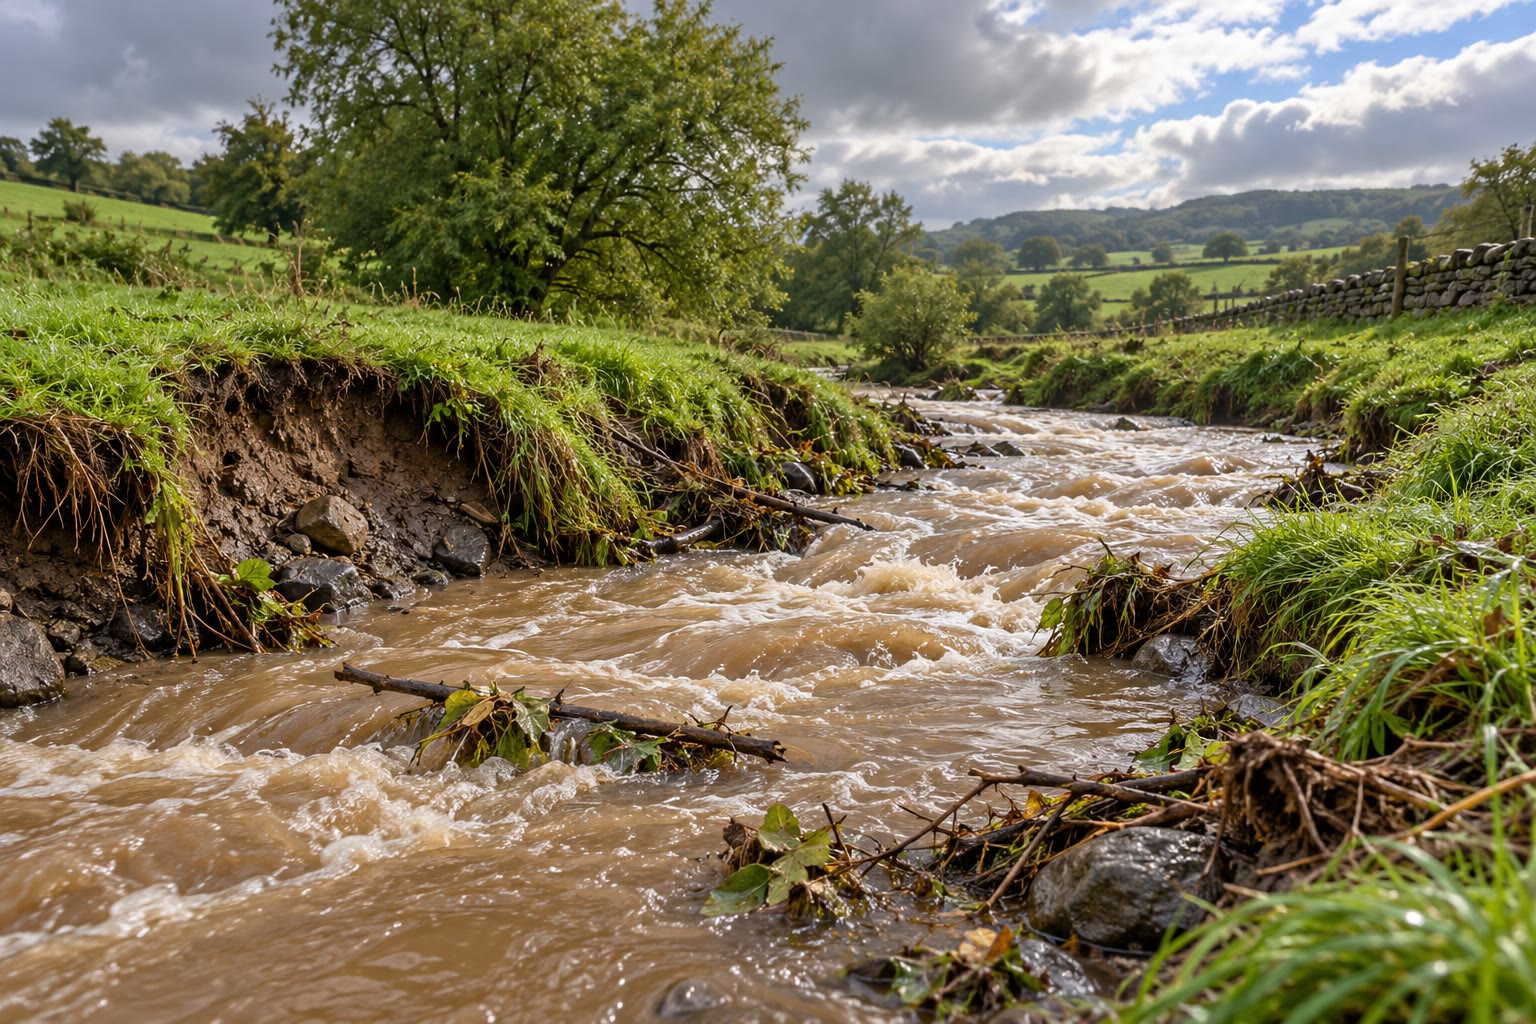
\includegraphics[width=0.5\linewidth]{images/book1/ai/g5-brown-stream.jpg}

{\small Un arroyo la mañana después de una tormenta: el agua está marrón por
el \omterm{def:g3:stones-pebbles-sand:sand}{barro} y la \omterm{def:g3:stones-pebbles-sand:sand}{arena} que lleva.}
\end{omfigure}

\begin{recall}
La \omterm{def:g3:stones-pebbles-sand:rock}{roca} es el material duro de la Tierra; rota en trozos da piedras, \omterm{def:g3:stones-pebbles-sand:pebble}{cantos}
redondeados por el agua, \omterm{def:g3:stones-pebbles-sand:sand}{arena}, cuyos granos se ven uno a uno, y \omterm{def:g3:stones-pebbles-sand:sand}{barro},
cuyos granos son demasiado pequeños para verlos
(\cref{ch:g3:stones-pebbles-sand}). Un \omterm{def:g1:landscapes-around-us:water}{río} corre todo el tiempo por un
cauce largo, desde las tierras más altas hasta un \omterm{def:g1:landscapes-around-us:water}{lago} o hasta el \omterm{def:g2:water-on-earth:ocean}{mar}
(\cref{ch:g1:landscapes-around-us}). La \omterm{def:g4:clouds-rain-snow:precipitation}{lluvia} que cae sobre la tierra
corre hasta los arroyos y los \omterm{def:g1:landscapes-around-us:water}{ríos}, que devuelven el agua al \omterm{def:g2:water-on-earth:ocean}{mar}
(\cref{ch:g2:water-on-earth}).
\end{recall}

\section{La roca se rompe donde está}

Ni siquiera la \omterm{def:g3:stones-pebbles-sand:rock}{roca} más dura dura para siempre. Donde está al descubierto,
bajo el sol, la \omterm{def:g4:clouds-rain-snow:precipitation}{lluvia} y las heladas, se agrieta y se desmorona poco a
poco.

\begin{definition}[Meteorización]\label{def:g5:water-shapes-the-land:weathering}
La \emph{meteorización}\index{meteorizacion@meteorización} es la rotura
lenta de la \omterm{def:g3:stones-pebbles-sand:rock}{roca} en el mismo lugar donde está, por la helada, el agua, las
raíces de las plantas y el calor y el frío. La \omterm{def:g3:stones-pebbles-sand:rock}{roca} se rompe en trozos,
pero los trozos se quedan en su sitio.
\end{definition}

La helada es una de las herramientas más fuertes de la \omterm{def:g5:water-shapes-the-land:weathering}{meteorización}. El
agua de \omterm{def:g4:clouds-rain-snow:precipitation}{lluvia} se mete en una grieta fina de la \omterm{def:g3:stones-pebbles-sand:rock}{roca}. Una noche fría se
congela, y cuando el agua se congela ocupa un poco más de sitio: el hielo
empuja las paredes de la grieta y la abre un poquito más. Al día siguiente
el hielo se funde, entra más agua, y a la noche siguiente vuelve a
congelarse. Después de muchos inviernos, se desprende un trozo de \omterm{def:g3:stones-pebbles-sand:rock}{roca}.

\begin{omfigure}
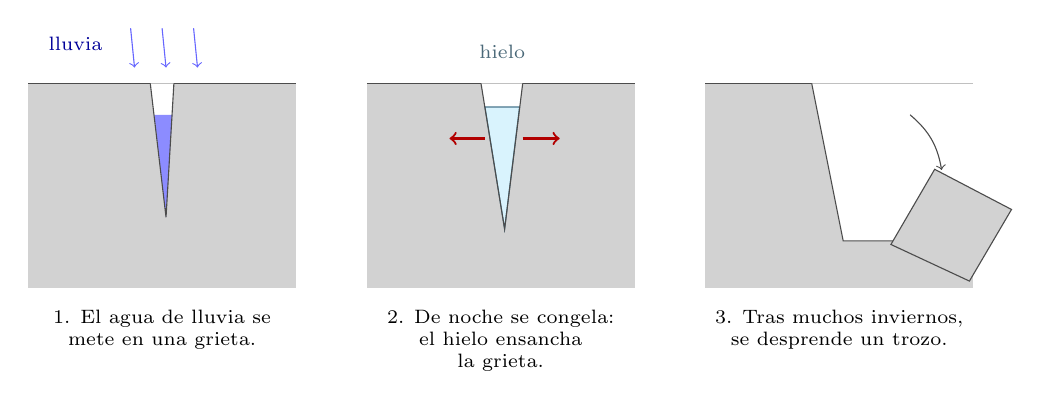
\begin{tikzpicture}[x=1cm, y=1cm, font=\scriptsize]
  \foreach \i/\t in {0/{1. El agua de lluvia se\\mete en una grieta.},
                     4.3/{2. De noche se congela:\\el hielo ensancha\\la grieta.},
                     8.6/{3. Tras muchos inviernos,\\se desprende un trozo.}} {
    \begin{scope}[xshift=\i cm]
      \fill[gray!35] (0,0) rectangle (3.4,2.6);
      \draw[gray!60!black] (0,2.6) -- (3.4,2.6);
      \node[align=center, anchor=north] at (1.7,-0.15) {\t};
    \end{scope}
  }
  % panel 1: thin crack with water
  \fill[white] (1.55,2.6) -- (1.75,0.9) -- (1.85,2.6) -- cycle;
  \fill[blue!45] (1.6,2.2) -- (1.75,0.9) -- (1.83,2.2) -- cycle;
  \draw[gray!60!black] (1.55,2.6) -- (1.75,0.9) -- (1.85,2.6);
  \foreach \x in {1.3,1.7,2.1} \draw[blue!60, ->] (\x,3.3) -- (\x+0.05,2.8);
  \node[blue!60!black] at (0.6,3.1) {lluvia};
  % panel 2: wider crack with ice
  \begin{scope}[xshift=4.3cm]
    \fill[white] (1.45,2.6) -- (1.75,0.75) -- (1.98,2.6) -- cycle;
    \fill[cyan!15] (1.5,2.3) -- (1.75,0.75) -- (1.94,2.3) -- cycle;
    \draw[cyan!50!black] (1.5,2.3) -- (1.75,0.75) -- (1.94,2.3) -- cycle;
    \draw[gray!60!black] (1.45,2.6) -- (1.75,0.75) -- (1.98,2.6);
    \draw[red!70!black, thick, <-] (1.05,1.9) -- (1.5,1.9);
    \draw[red!70!black, thick, ->] (1.98,1.9) -- (2.45,1.9);
    \node[cyan!40!black] at (1.72,3.0) {hielo};
  \end{scope}
  % panel 3: broken block
  \begin{scope}[xshift=8.6cm]
    \fill[white] (1.35,2.6) -- (1.75,0.6) -- (3.4,0.6) -- (3.4,2.6) -- cycle;
    \draw[gray!60!black] (1.35,2.6) -- (1.75,0.6) -- (3.4,0.6);
    \fill[gray!35, draw=gray!60!black, rotate around={-25:(2.9,0.3)}]
      (2.3,0.3) -- (2.4,1.4) -- (3.5,1.35) -- (3.4,0.3) -- cycle;
    \draw[gray!60!black, ->] (2.6,2.2) to[bend left=20] (3.0,1.5);
  \end{scope}
\end{tikzpicture}

{\small La helada rompe la \omterm{def:g3:stones-pebbles-sand:rock}{roca}. Cada noche de helada, el hielo de una
grieta empuja un poco; después de muchos inviernos, la grieta es lo bastante
ancha para que se desprenda un trozo.}
\end{omfigure}

Al pie de un cortado de \omterm{def:g3:stones-pebbles-sand:rock}{roca} desnuda, en lo alto de las \omterm{def:g1:landscapes-around-us:landform}{montañas}, los
trozos desprendidos por la helada resbalan y ruedan ladera abajo, y se
amontonan en una pendiente de piedras afiladas. No están redondeadas:
ningún agua las ha hecho rodar todavía.

\begin{omfigure}
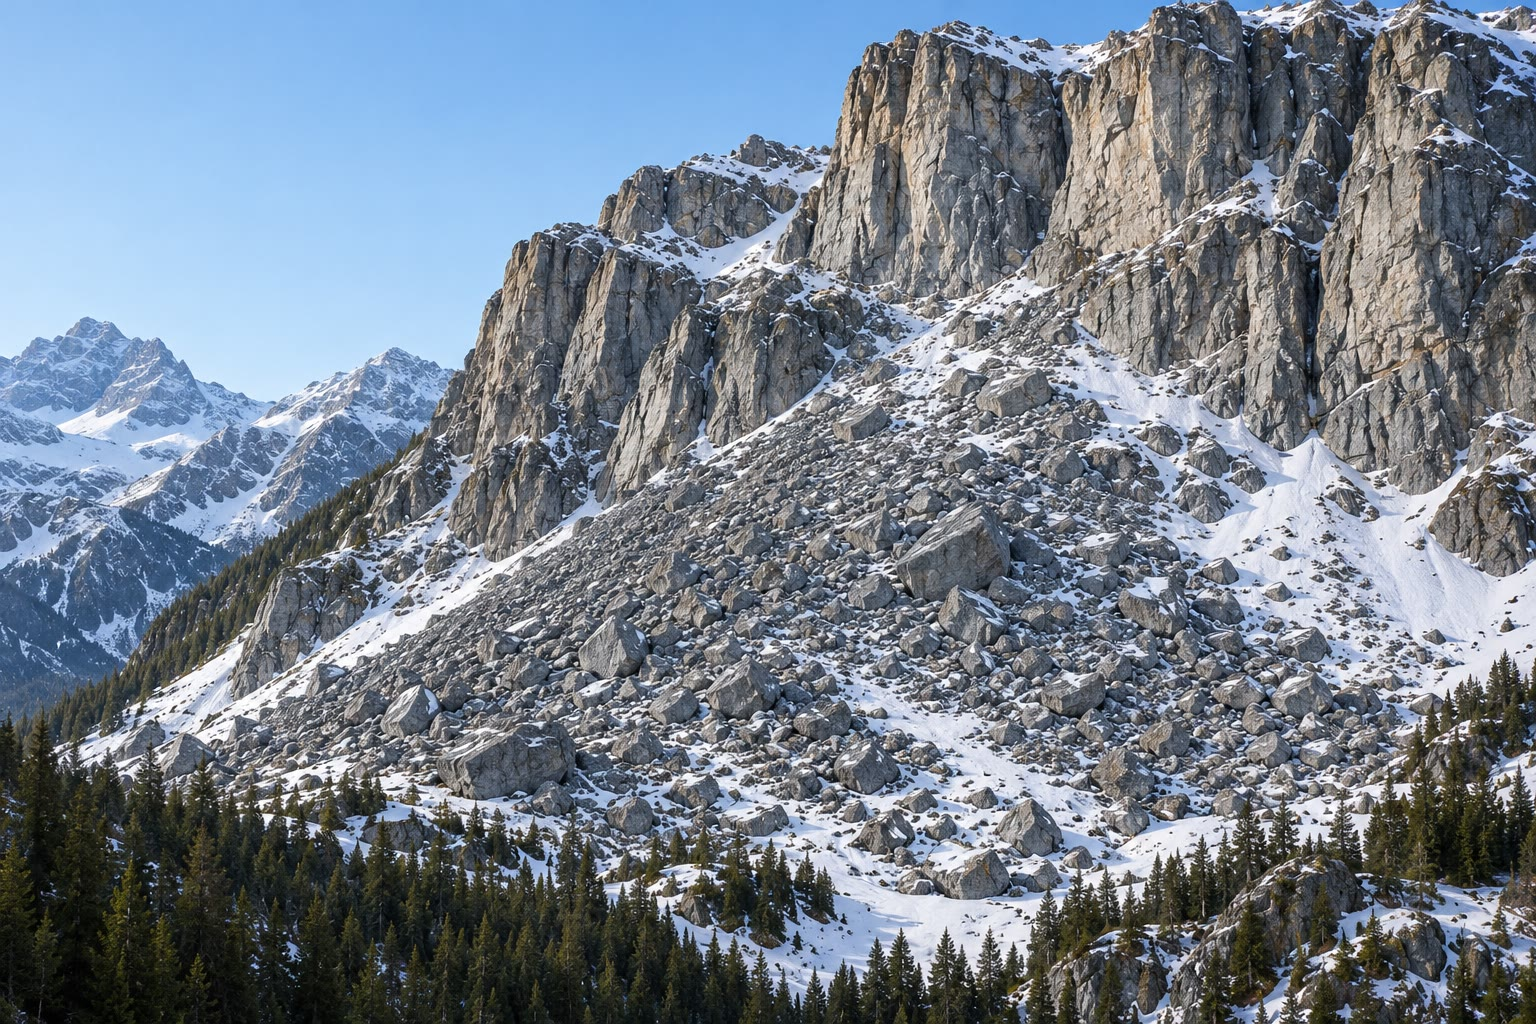
\includegraphics[width=0.5\linewidth]{images/book1/ai/g5-frost-scree.jpg}

{\small Al pie de un cortado de \omterm{def:g1:landscapes-around-us:landform}{montaña}, una pendiente de piedras de
aristas vivas desprendidas por la helada, vista desde el otro lado del
\omterm{def:g1:landscapes-around-us:landform}{valle}.}
\end{omfigure}

Las plantas también ayudan. Una raíz de árbol se cuela en una grieta y, al
engordar año tras año, parte la \omterm{def:g3:stones-pebbles-sand:rock}{roca} como una cuña lenta. El propio agua
de \omterm{def:g4:clouds-rain-snow:precipitation}{lluvia} ablanda poco a poco algunas \omterm{def:g3:stones-pebbles-sand:rock}{rocas} y las convierte en arcilla y
\omterm{def:g3:stones-pebbles-sand:sand}{arena}: así consigue el suelo sus granos minerales.

\section{El agua se lleva los trozos}

Una vez rota la \omterm{def:g3:stones-pebbles-sand:rock}{roca}, los trozos pueden moverse. Algo tiene que llevarlos.

\begin{definition}[Erosión]\label{def:g5:water-shapes-the-land:erosion}
La \emph{erosión}\index{erosion@erosión} es el desgaste del terreno y el
arrastre de los trozos de \omterm{def:g3:stones-pebbles-sand:rock}{roca}, sobre todo por el agua que corre, pero
también por el viento, el hielo y las olas del \omterm{def:g2:water-on-earth:ocean}{mar}.
\end{definition}

El agua que corre hace casi todo el trabajo. La \omterm{def:g4:clouds-rain-snow:precipitation}{lluvia} arrastra tierra y
granos ladera abajo hasta los arroyos; los arroyos arrancan más de sus
propias orillas, como hizo el arroyo de Tom y Lena después de la tormenta.
Cuanto más deprisa corre el agua, más puede llevar, y más grandes son los
trozos que puede mover: un arroyo tranquilo solo lleva \omterm{def:g3:stones-pebbles-sand:sand}{barro} fino; un
arroyo crecido hace rodar \omterm{def:g3:stones-pebbles-sand:pebble}{cantos} e incluso bloques por su lecho.

Por el camino, las piedras chocan entre sí y contra el lecho. Se les rompen
las esquinas y se convierten en \omterm{def:g3:stones-pebbles-sand:pebble}{cantos} redondeados, y luego en granos cada
vez más pequeños: \omterm{def:g3:stones-pebbles-sand:sand}{arena} y \omterm{def:g3:stones-pebbles-sand:sand}{barro}.

El viento hace el mismo trabajo en los lugares secos, donde nada sujeta la
\omterm{def:g3:stones-pebbles-sand:sand}{arena}: la empuja y forma dunas. El hielo, en las \omterm{def:g1:landscapes-around-us:landform}{montañas} y cerca de los
\omterm{def:g3:continents-and-oceans:poles}{polos}, arrastra piedras bajo su enorme peso. En la \omterm{def:g1:landscapes-around-us:water}{costa}, las olas golpean
los acantilados y hacen rodar los \omterm{def:g3:stones-pebbles-sand:pebble}{cantos} de la playa de un lado a otro.

\begin{remark}[¿Cuánto?]\label{rem:g5:water-shapes-the-land:how-much}
Entre todos, los \omterm{def:g1:landscapes-around-us:water}{ríos} del mundo llevan al \omterm{def:g2:water-on-earth:ocean}{mar} más de 12\,000 millones de
toneladas de \omterm{def:g3:stones-pebbles-sand:sand}{barro} y \omterm{def:g3:stones-pebbles-sand:sand}{arena} cada año. Son unos mil millones de toneladas
cada mes.
% ledger: syvitski:modern-flux
\end{remark}

\section{El agua deja los trozos}

Un \omterm{def:g1:landscapes-around-us:water}{río} no puede llevar su carga para siempre. Donde se frena, ya no tiene
fuerza para mover sus granos más grandes, y estos se depositan en el lecho.

\begin{definition}[Sedimentación]\label{def:g5:water-shapes-the-land:deposition}
La \emph{sedimentación}\index{sedimentacion@sedimentación} es el depósito
de los trozos de \omterm{def:g3:stones-pebbles-sand:rock}{roca} que llevan el agua, el viento o el hielo, allí donde
se frenan y se detienen.
\end{definition}

Los trozos más pesados se depositan primero: los \omterm{def:g3:stones-pebbles-sand:pebble}{cantos} caen donde la
corriente afloja un poco, la \omterm{def:g3:stones-pebbles-sand:sand}{arena} donde se frena más, y el \omterm{def:g3:stones-pebbles-sand:sand}{barro} fino solo
donde el agua está casi quieta, en un \omterm{def:g1:landscapes-around-us:water}{lago} o en el \omterm{def:g2:water-on-earth:ocean}{mar}. Por eso el lecho de
un \omterm{def:g1:landscapes-around-us:water}{río} es pedregoso en las \omterm{def:g1:landscapes-around-us:landform}{montañas} y arenoso o fangoso cerca del \omterm{def:g2:water-on-earth:ocean}{mar}.

La \omterm{def:g5:water-shapes-the-land:weathering}{meteorización}, la \omterm{def:g5:water-shapes-the-land:erosion}{erosión} y la \omterm{def:g5:water-shapes-the-land:deposition}{sedimentación} son tres etapas de un mismo
largo viaje: la \omterm{def:g3:stones-pebbles-sand:rock}{roca} se rompe donde está, sus trozos se van, y se depositan
en otro lugar. Poco a poco, el agua mueve las \omterm{def:g1:landscapes-around-us:landform}{montañas}, grano a grano,
hacia las \omterm{def:g1:landscapes-around-us:landform}{llanuras} y hasta el \omterm{def:g2:water-on-earth:ocean}{mar}.

\begin{method}[Poner nombre a lo que hace el agua]\label{met:g5:water-shapes-the-land:naming}
Para poner nombre a lo que le está pasando a la \omterm{def:g3:stones-pebbles-sand:rock}{roca} en una foto o en una
historia, hazte tres preguntas:
\begin{enumerate}
  \item ¿Se está rompiendo la \omterm{def:g3:stones-pebbles-sand:rock}{roca}, pero los trozos se quedan donde están?
        Eso es la \emph{\omterm{def:g5:water-shapes-the-land:weathering}{meteorización}}.
  \item ¿Se están desgastando los trozos y se los lleva algo? Eso es la
        \emph{\omterm{def:g5:water-shapes-the-land:erosion}{erosión}}.
  \item ¿Se están posando los trozos y se amontonan? Eso es la
        \emph{\omterm{def:g5:water-shapes-the-land:deposition}{sedimentación}}.
\end{enumerate}
\end{method}

\begin{example}[El arroyo después de la tormenta]\label{ex:g5:water-shapes-the-land:stream}
El agua marrón del arroyo de Tom y Lena lleva \omterm{def:g3:stones-pebbles-sand:sand}{barro} arrancado de sus
orillas: eso es \omterm{def:g5:water-shapes-the-land:erosion}{erosión}. Una semana después, el arroyo vuelve a estar
claro, y una capa fina de \omterm{def:g3:stones-pebbles-sand:sand}{barro} cubre el fondo de la poza tranquila del
final del patio: eso es \omterm{def:g5:water-shapes-the-land:deposition}{sedimentación}.
\end{example}

\section{Un río desde su nacimiento hasta su desembocadura}

Todo \omterm{def:g1:landscapes-around-us:water}{río} tiene un principio y un final.

\begin{definition}[Nacimiento, desembocadura y afluente]\label{def:g5:water-shapes-the-land:source-mouth}
El \emph{nacimiento}\index{nacimiento (de un rio)@nacimiento (de un río)}
de un \omterm{def:g1:landscapes-around-us:water}{río} es el lugar donde empieza: un manantial, un glaciar que se funde
o una tierra alta y húmeda donde nacen muchos arroyuelos. Su
\emph{desembocadura}\index{desembocadura} es el lugar donde termina, al
verter sus aguas en el \omterm{def:g2:water-on-earth:ocean}{mar}, en un \omterm{def:g1:landscapes-around-us:water}{lago} o en un \omterm{def:g1:landscapes-around-us:water}{río} más grande. Un
\emph{afluente}\index{afluente} es un \omterm{def:g1:landscapes-around-us:water}{río} más pequeño que desemboca en otro
más grande.
\end{definition}

A lo largo de su camino, un \omterm{def:g1:landscapes-around-us:water}{río} cambia. Dividimos su longitud en tres
partes: el curso alto, el curso medio y el curso bajo.

\begin{omfigure}
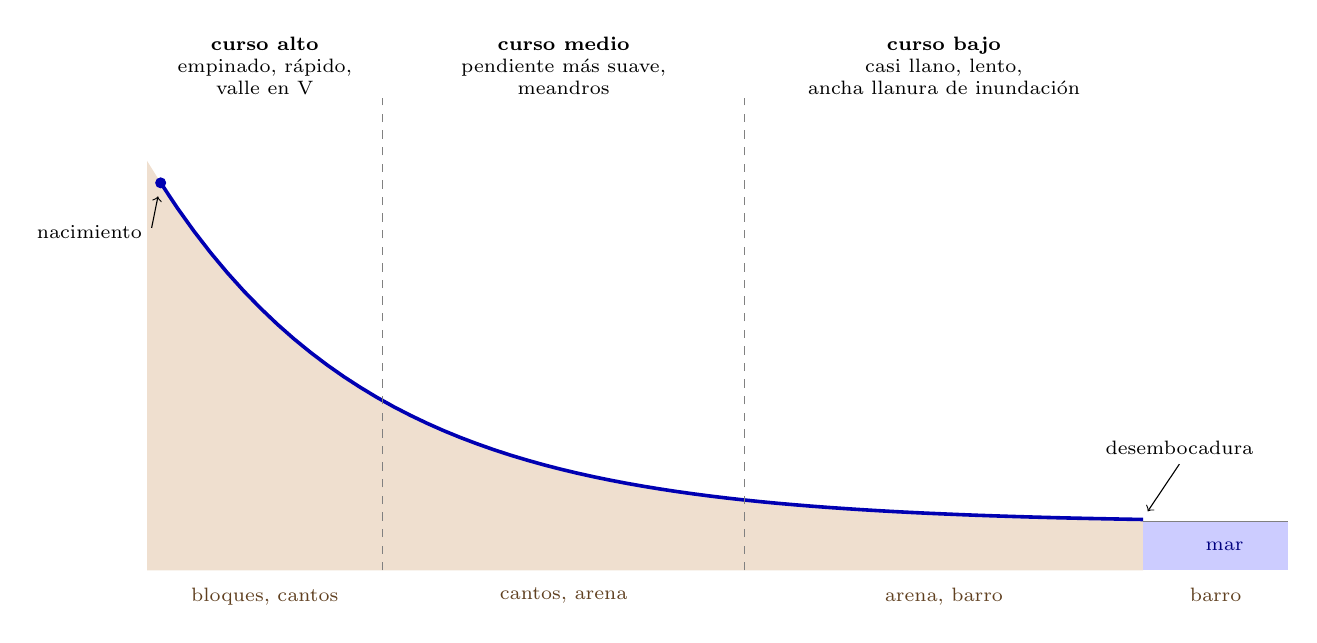
\begin{tikzpicture}[x=1.15cm, y=1cm, font=\scriptsize]
  % ground
  \fill[brown!25] (0,-0.6) -- plot[domain=0:11, samples=60]
    (\x,{4.6*exp(-\x/2.4)}) -- (11,-0.6) -- cycle;
  % sea
  \fill[blue!20] (11,-0.6) rectangle (12.6,0.02);
  \draw[blue!70!black, line width=1.3pt] plot[domain=0.15:11, samples=60]
    (\x,{4.6*exp(-\x/2.4)});
  \draw[gray] (11,0.02) -- (12.6,0.02);
  \node[blue!50!black] at (11.9,-0.3) {mar};
  % course limits
  \foreach \x in {2.6,6.6} \draw[gray, dashed] (\x,-0.6) -- (\x,5.4);
  \node[align=center, anchor=north] at (1.3,6.3) {\textbf{curso alto}\\empinado, rápido,\\valle en V};
  \node[align=center, anchor=north] at (4.6,6.3) {\textbf{curso medio}\\pendiente más suave,\\meandros};
  \node[align=center, anchor=north] at (8.8,6.3) {\textbf{curso bajo}\\casi llano, lento,\\ancha llanura de inundación};
  % source and mouth
  \fill[blue!70!black] (0.15,{4.6*exp(-0.15/2.4)}) circle (2pt);
  \node[anchor=east] at (0.05,3.7) {nacimiento};
  \draw[->] (0.05,3.75) -- (0.12,4.15);
  \node[anchor=south] at (11.4,0.75) {desembocadura};
  \draw[->] (11.4,0.75) -- (11.05,0.15);
  % grain sizes
  \node[anchor=north, align=center, text=brown!50!black] at (1.3,-0.7) {bloques, cantos};
  \node[anchor=north, align=center, text=brown!50!black] at (4.6,-0.7) {cantos, arena};
  \node[anchor=north, align=center, text=brown!50!black] at (8.8,-0.7) {arena, barro};
  \node[anchor=north, align=center, text=brown!50!black] at (11.8,-0.7) {barro};
\end{tikzpicture}

{\small El perfil longitudinal de un \omterm{def:g1:landscapes-around-us:water}{río}, desde su \omterm{def:g5:water-shapes-the-land:source-mouth}{nacimiento} hasta su
\omterm{def:g5:water-shapes-the-land:source-mouth}{desembocadura} (las alturas están muy exageradas). Debajo: lo que hay en su
lecho.}
\end{omfigure}

En su \emph{curso alto}, en las \omterm{def:g1:landscapes-around-us:landform}{montañas}, el \omterm{def:g1:landscapes-around-us:water}{río} es joven y empinado. Su
agua baja con fuerza, hace rodar bloques por su lecho y excava hacia abajo
en la \omterm{def:g3:stones-pebbles-sand:rock}{roca}. Abre un \omterm{def:g1:landscapes-around-us:landform}{valle} estrecho de laderas empinadas, con la forma de la
letra V.

En su \emph{curso medio}, la pendiente es más suave. El \omterm{def:g1:landscapes-around-us:water}{río} va de un lado a
otro formando grandes curvas.

\begin{definition}[Meandro]\label{def:g5:water-shapes-the-land:meander}
Un \emph{meandro}\index{meandro} es una curva de un \omterm{def:g1:landscapes-around-us:water}{río} que serpentea por
el fondo llano de un \omterm{def:g1:landscapes-around-us:landform}{valle}.
\end{definition}

Un \omterm{def:g5:water-shapes-the-land:meander}{meandro} no se queda quieto: se desplaza. En la parte de fuera de cada
curva, el agua corre deprisa y es profunda: va comiéndose la orilla, que se
convierte en un pequeño cortado. En la parte de dentro de la curva, el agua
corre despacio: deja \omterm{def:g3:stones-pebbles-sand:sand}{arena} y \omterm{def:g3:stones-pebbles-sand:pebble}{grava}, que forman una playa suave. Año tras
año, la orilla de fuera retrocede y la playa de dentro crece, y la curva se
abre cada vez más.

\begin{omfigure}
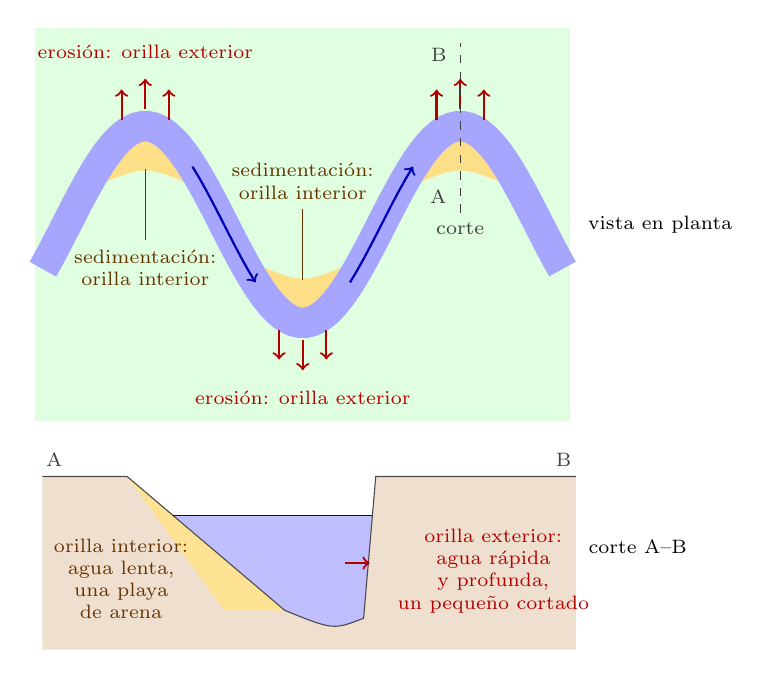
\begin{tikzpicture}[x=1cm, y=1cm, font=\scriptsize]
  % ---- map view ----
  \fill[green!12] (-0.4,-2.5) rectangle (6.4,2.5);
  % sand on the inner banks (drawn first, the river covers its edge)
  \foreach \c/\s in {1/1, 3/-1, 5/1}
    \fill[yellow!50!orange!45] (\c-0.6,\s*0.5) .. controls (\c,\s*1.5) ..
      (\c+0.6,\s*0.5) .. controls (\c,\s*0.75) .. cycle;
  % the river
  \draw[blue!35, line width=11pt] plot[domain=-0.3:6.3, samples=90]
    (\x,{1.25*sin(\x*90)});
  \draw[blue!70!black, ->, thick] plot[domain=1.6:2.4, samples=10]
    (\x,{1.25*sin(\x*90)});
  \draw[blue!70!black, ->, thick] plot[domain=3.6:4.4, samples=10]
    (\x,{1.25*sin(\x*90)});
  % erosion on the outer banks
  \foreach \c/\s in {1/1, 3/-1, 5/1}
    \foreach \d in {-0.3,0,0.3}
      \draw[red!70!black, thick, ->] (\c+\d,{\s*(1.25*cos(\d*90)+0.22)})
        -- (\c+\d,{\s*(1.25*cos(\d*90)+0.6)});
  \node[red!70!black] at (1,2.2) {erosión: orilla exterior};
  \node[red!70!black] at (3,-2.2) {erosión: orilla exterior};
  \node[orange!40!black, align=center] (d1) at (1,-0.55) {sedimentación:\\orilla interior};
  \node[orange!40!black, align=center] (d2) at (3,0.55) {sedimentación:\\orilla interior};
  \draw[orange!40!black] (d1.north) -- (1,0.7);
  \draw[orange!40!black] (d2.south) -- (3,-0.7);
  \draw[gray!50!black, dashed] (5,0.15) -- (5,2.3);
  \node[gray!50!black, anchor=north] at (5,0.15) {corte};
  \node[gray!50!black, anchor=east] at (4.95,0.35) {A};
  \node[gray!50!black, anchor=east] at (4.95,2.15) {B};
  \node[anchor=west] at (6.5,0) {vista en planta};
  % ---- cut ----
  \begin{scope}[yshift=-4.1cm, xscale=0.77]
    \fill[brown!25] (-0.4,-1.3) -- (-0.4,0.9) -- (1,0.9) -- (3.6,-0.8)
      .. controls (4.4,-1.05) .. (4.9,-0.9) -- (5.1,0.9) -- (8.4,0.9)
      -- (8.4,-1.3) -- cycle;
    \fill[blue!25] (1.75,0.4) -- (3.6,-0.8) .. controls (4.4,-1.05) .. (4.9,-0.9)
      -- (5.04,0.4) -- cycle;
    \fill[yellow!50!orange!40] (1,0.9) -- (3.6,-0.8) -- (2.6,-0.8) -- cycle;
    \draw[gray!60!black] (-0.4,0.9) -- (1,0.9) -- (3.6,-0.8)
      .. controls (4.4,-1.05) .. (4.9,-0.9) -- (5.1,0.9) -- (8.4,0.9);
    \draw[blue!60!black] (1.75,0.4) -- (5.04,0.4);
    \node[orange!40!black, align=center] at (0.9,-0.4) {orilla interior:\\agua lenta,\\una playa\\de arena};
    \node[red!70!black, align=center, anchor=west] at (5.3,-0.3) {orilla exterior:\\agua rápida\\y profunda,\\un pequeño cortado};
    \draw[red!70!black, thick, ->] (4.6,-0.2) -- (5.0,-0.2);
    \node[gray!50!black, anchor=south] at (-0.2,0.9) {A};
    \node[gray!50!black, anchor=south] at (8.2,0.9) {B};
    \node[anchor=west] at (8.45,0) {corte A--B};
  \end{scope}
\end{tikzpicture}

{\small Un \omterm{def:g5:water-shapes-the-land:meander}{meandro} visto desde arriba, y cortado de través por la línea
discontinua A--B. El agua desgasta la orilla exterior de cada curva y deja
\omterm{def:g3:stones-pebbles-sand:sand}{arena} en la orilla interior: la curva se desplaza poco a poco.}
\end{omfigure}

A veces dos curvas crecen tanto que se acercan y, durante una \omterm{def:g5:water-shapes-the-land:flood}{crecida}, el
\omterm{def:g1:landscapes-around-us:water}{río} rompe el estrecho cuello de tierra que las separa y toma el atajo. La
curva vieja se queda atrás convertida en un \omterm{def:g1:landscapes-around-us:water}{lago} curvo.

\begin{omfigure}
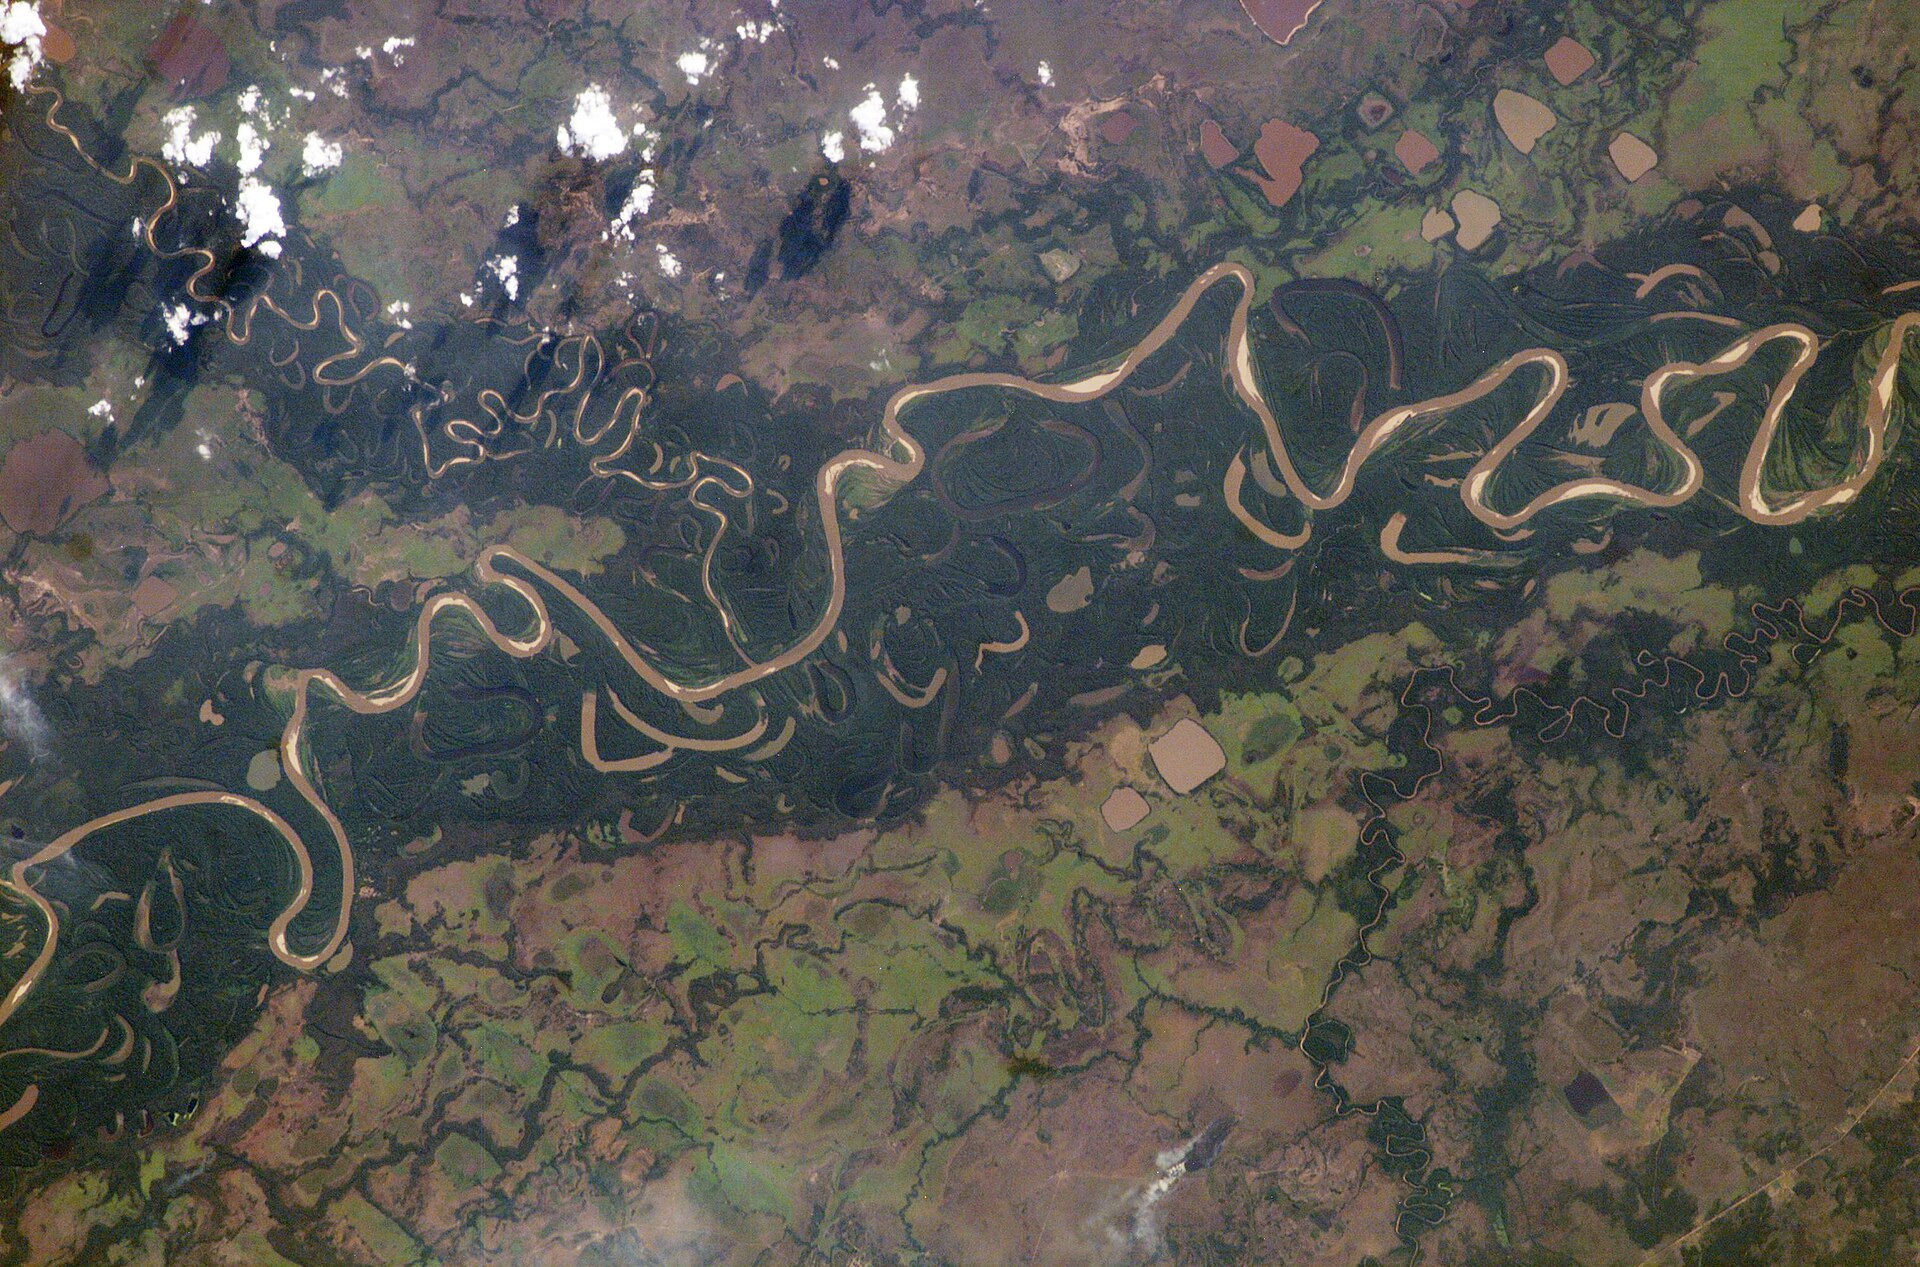
\includegraphics[width=0.52\linewidth]{images/book1/g5-mamore-meanders.jpg}

{\small El \omterm{def:g1:landscapes-around-us:water}{río} Mamoré, en las tierras bajas de Bolivia, en América del Sur,
visto desde la Estación Espacial Internacional. El \omterm{def:g1:landscapes-around-us:water}{río} marrón serpentea en
\omterm{def:g5:water-shapes-the-land:meander}{meandros} a través de la selva. Fotografía: NASA (dominio
público).}\label{fig:g5:water-shapes-the-land:mamore}
% ledger: nasa:mamore-meanders
\end{omfigure}

En su \emph{curso bajo}, la tierra es casi llana. El \omterm{def:g1:landscapes-around-us:water}{río} corre despacio por
el fondo ancho y llano de un \omterm{def:g1:landscapes-around-us:landform}{valle}, hecho del \omterm{def:g3:stones-pebbles-sand:sand}{barro} y la \omterm{def:g3:stones-pebbles-sand:sand}{arena} que él mismo
ha ido dejando durante muchísimo tiempo.

\begin{omfigure}
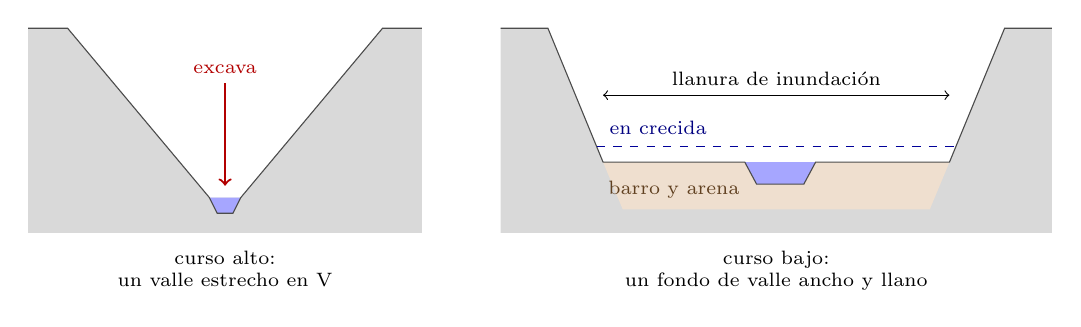
\begin{tikzpicture}[x=1cm, y=1cm, font=\scriptsize]
  % V-shaped valley
  \fill[gray!30] (0,0) -- (0,2.6) -- (0.5,2.6) -- (2.3,0.45) -- (2.7,0.45)
    -- (4.5,2.6) -- (5,2.6) -- (5,0) -- cycle;
  \fill[blue!35] (2.3,0.45) -- (2.4,0.25) -- (2.6,0.25) -- (2.7,0.45) -- cycle;
  \draw[gray!60!black] (0,2.6) -- (0.5,2.6) -- (2.3,0.45) -- (2.4,0.25)
    -- (2.6,0.25) -- (2.7,0.45) -- (4.5,2.6) -- (5,2.6);
  \draw[red!70!black, thick, ->] (2.5,1.9) -- (2.5,0.6);
  \node[red!70!black, anchor=south] at (2.5,1.9) {excava};
  \node[align=center, anchor=north] at (2.5,-0.1) {curso alto:\\un valle estrecho en V};
  % floodplain
  \begin{scope}[xshift=6cm]
    \fill[gray!30] (0,0) -- (0,2.6) -- (0.6,2.6) -- (1.3,0.9) -- (5.7,0.9)
      -- (6.4,2.6) -- (7,2.6) -- (7,0) -- cycle;
    \fill[brown!25] (1.3,0.9) -- (1.55,0.3) -- (5.45,0.3) -- (5.7,0.9) -- cycle;
    \fill[blue!35] (3.1,0.9) -- (3.25,0.62) -- (3.85,0.62) -- (4,0.9) -- cycle;
    \draw[gray!60!black] (0,2.6) -- (0.6,2.6) -- (1.3,0.9) -- (3.1,0.9)
      -- (3.25,0.62) -- (3.85,0.62) -- (4,0.9) -- (5.7,0.9) -- (6.4,2.6) -- (7,2.6);
    \draw[blue!60!black, dashed] (1.22,1.1) -- (5.78,1.1);
    \node[blue!50!black, anchor=south] at (2.0,1.12) {en crecida};
    \node[brown!50!black] at (2.2,0.55) {barro y arena};
    \draw[<->] (1.3,1.75) -- (5.7,1.75);
    \node[anchor=south] at (3.5,1.75) {llanura de inundación};
    \node[align=center, anchor=north] at (3.5,-0.1) {curso bajo:\\un fondo de valle ancho y llano};
  \end{scope}
\end{tikzpicture}

{\small El \omterm{def:g1:landscapes-around-us:landform}{valle} cortado de través, en las \omterm{def:g1:landscapes-around-us:landform}{montañas} y cerca del \omterm{def:g2:water-on-earth:ocean}{mar} (no a la
misma escala). En las \omterm{def:g5:water-shapes-the-land:flood}{crecidas}, el \omterm{def:g1:landscapes-around-us:water}{río} se extiende por toda su \omterm{def:g5:water-shapes-the-land:flood}{llanura de
inundación}.}
\end{omfigure}

Por fin el \omterm{def:g1:landscapes-around-us:water}{río} llega a su \omterm{def:g5:water-shapes-the-land:source-mouth}{desembocadura}. Allí el agua se frena casi del
todo, y el \omterm{def:g1:landscapes-around-us:water}{río} deja lo último de su carga. Donde las olas y las mareas del
\omterm{def:g2:water-on-earth:ocean}{mar} son demasiado débiles para llevárselo todo, el \omterm{def:g3:stones-pebbles-sand:sand}{barro} y la \omterm{def:g3:stones-pebbles-sand:sand}{arena} se
amontonan, y nace tierra nueva que avanza sobre el \omterm{def:g2:water-on-earth:ocean}{mar}.

\begin{definition}[Delta]\label{def:g5:water-shapes-the-land:delta}
Un \emph{delta}\index{delta} es una tierra nueva y llana que un \omterm{def:g1:landscapes-around-us:water}{río}
construye en su \omterm{def:g5:water-shapes-the-land:source-mouth}{desembocadura} con el \omterm{def:g3:stones-pebbles-sand:sand}{barro} y la \omterm{def:g3:stones-pebbles-sand:sand}{arena} que deja. El \omterm{def:g1:landscapes-around-us:water}{río} se
divide en varios brazos que se abren sobre ella, a menudo en forma de
abanico.
\end{definition}

El nombre viene de la letra griega $\Delta$ (\omterm{def:g5:water-shapes-the-land:delta}{delta}), un triángulo, porque
el \omterm{def:g5:water-shapes-the-land:delta}{delta} del Nilo, en Egipto, tiene esa forma.

Algunos \omterm{def:g1:landscapes-around-us:water}{ríos} terminan sin \omterm{def:g5:water-shapes-the-land:delta}{delta}. Donde unas olas y unas mareas fuertes se
llevan el \omterm{def:g3:stones-pebbles-sand:sand}{barro}, el \omterm{def:g1:landscapes-around-us:water}{río} termina en una \omterm{def:g5:water-shapes-the-land:source-mouth}{desembocadura} ancha, en forma de
embudo, por donde el \omterm{def:g2:water-on-earth:ocean}{mar} entra y sale con las mareas: un \emph{estuario}.

\begin{omfigure}
\begin{minipage}[b]{0.55\linewidth}\centering
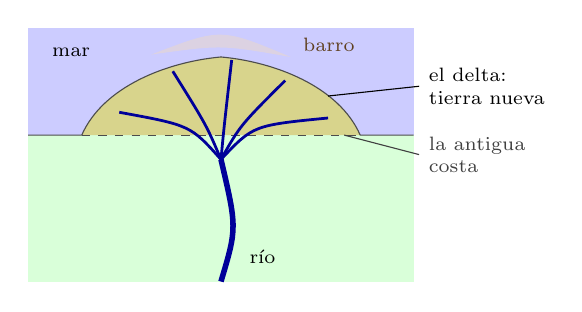
\begin{tikzpicture}[x=0.68cm, y=0.62cm, font=\scriptsize]
  \fill[blue!20] (-3.6,1.4) rectangle (3.6,3.6);
  \fill[green!15] (-3.6,-1.6) rectangle (3.6,1.4);
  % delta
  \fill[olive!35] (-2.6,1.4) .. controls (-2.2,2.4) and (-1,2.9)
    .. (0,3.0) .. controls (1,2.9) and (2.2,2.4) .. (2.6,1.4) -- cycle;
  \draw[gray!60!black] (-3.6,1.4) -- (-2.6,1.4) .. controls (-2.2,2.4) and
    (-1,2.9) .. (0,3.0) .. controls (1,2.9) and (2.2,2.4) .. (2.6,1.4) -- (3.6,1.4);
  \draw[gray!60!black, dashed] (-2.6,1.4) -- (2.6,1.4);
  % river and branches
  \draw[blue!60!black, line width=2pt] (0,-1.6) .. controls (0.3,-0.5) .. (0,0.9);
  \foreach \e in {-1.9,-0.9,0.2,1.2,2.0}
    \draw[blue!60!black, line width=1pt] (0,0.9) .. controls (\e*0.3,1.6) ..
      (\e,{2.95-0.3*\e*\e});
  % mud plume
  \fill[brown!30, opacity=0.5] (-1.3,3.05) .. controls (0,3.6) .. (1.3,3.0)
    .. controls (0,3.25) .. cycle;
  \node[align=center] at (-2.8,3.1) {mar};
  \node[anchor=west, brown!50!black] at (1.35,3.25) {barro};
  \node[anchor=west, align=left] at (3.7,2.4) {el delta:\\tierra nueva};
  \draw (3.7,2.4) -- (2.0,2.2);
  \node[anchor=west, align=left, gray!50!black] at (3.7,1.0) {la antigua\\costa};
  \draw[gray!50!black] (3.7,1.0) -- (2.3,1.4);
  \node[anchor=west] at (0.35,-1.1) {río};
\end{tikzpicture}
\end{minipage}\hfill
\begin{minipage}[b]{0.3\linewidth}\centering
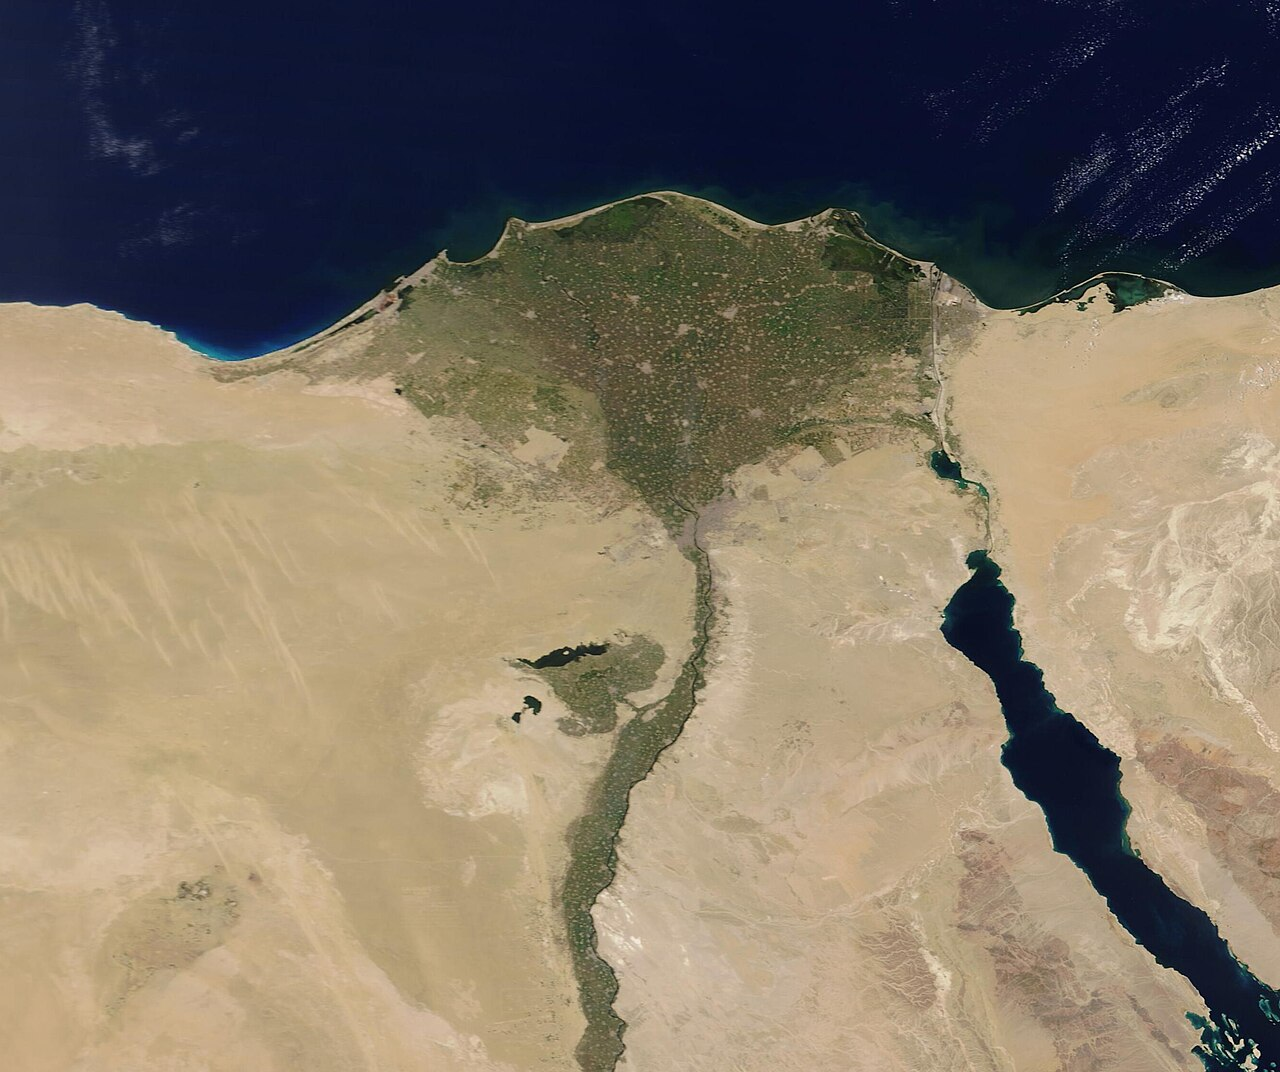
\includegraphics[width=\linewidth]{images/book1/g5-nile-delta-modis.jpg}
\end{minipage}

{\small A la izquierda, un \omterm{def:g5:water-shapes-the-land:delta}{delta} visto desde arriba; el \omterm{def:g3:stones-pebbles-sand:sand}{barro} y la \omterm{def:g3:stones-pebbles-sand:sand}{arena} que
dejan los brazos construyen tierra nueva más allá de la antigua \omterm{def:g1:landscapes-around-us:water}{costa}. A la
derecha, el \omterm{def:g5:water-shapes-the-land:delta}{delta} del Nilo, en Egipto, visto desde un satélite (el \omterm{def:g2:water-on-earth:ocean}{mar},
arriba): un abanico verde de campos sobre el \omterm{def:g3:stones-pebbles-sand:sand}{barro} del \omterm{def:g1:landscapes-around-us:water}{río}, en medio del
desierto. Fotografía: NASA (dominio público).}
% ledger: nasa:nile-delta-modis
\end{omfigure}

\section{Las inundaciones}

Después de muchos días de \omterm{def:g4:clouds-rain-snow:precipitation}{lluvia}, o cuando la \omterm{def:g4:clouds-rain-snow:precipitation}{nieve} se funde deprisa en
primavera, un \omterm{def:g1:landscapes-around-us:water}{río} recibe más agua de la que cabe en su cauce.

\begin{definition}[Inundación y llanura de inundación]\label{def:g5:water-shapes-the-land:flood}
Hay una \emph{inundación}\index{inundacion@inundación} cuando el agua
cubre una tierra que normalmente está seca. Un \omterm{def:g1:landscapes-around-us:water}{río} se desborda cuando sube
por encima de sus orillas y se extiende por la tierra llana que tiene a
cada lado. Esa tierra llana, que el \omterm{def:g1:landscapes-around-us:water}{río} cubre de vez en cuando, es su
\emph{llanura de inundación}\index{llanura de inundacion@llanura de inundación}.
\end{definition}

\begin{omfigure}
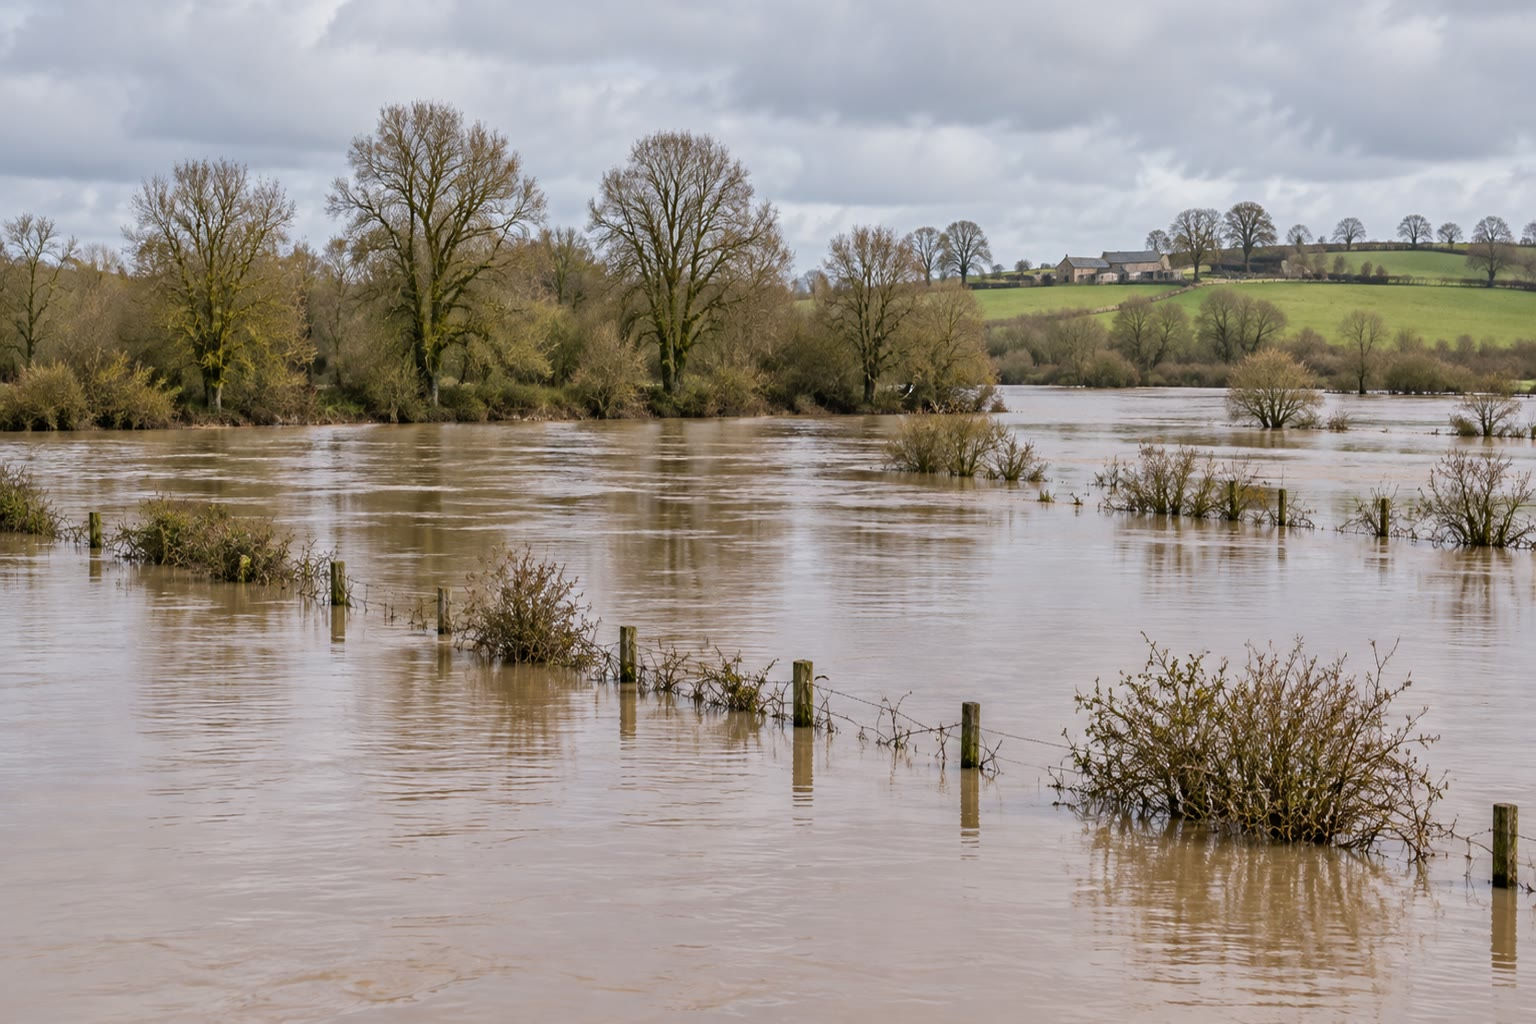
\includegraphics[width=0.5\linewidth]{images/book1/ai/g5-flooded-meadow.jpg}

{\small Un prado inundado después de varios días de \omterm{def:g4:clouds-rain-snow:precipitation}{lluvia}. La fila de
árboles marca la orilla habitual del \omterm{def:g1:landscapes-around-us:water}{río}; la granja está en un terreno más
alto.}
\end{omfigure}

Un \omterm{def:g1:landscapes-around-us:water}{río} que se desborda no hace nada raro: hace lo que los \omterm{def:g1:landscapes-around-us:water}{ríos} han hecho
siempre. La \omterm{def:g5:water-shapes-the-land:flood}{llanura de inundación} es su territorio. De hecho, la ha
construido el propio \omterm{def:g1:landscapes-around-us:water}{río}: cada \omterm{def:g5:water-shapes-the-land:flood}{crecida} deja una capa fina de \omterm{def:g3:stones-pebbles-sand:sand}{barro} sobre
los campos, y por eso las \omterm{def:g5:water-shapes-the-land:flood}{llanuras de inundación} tienen un suelo tan
fértil. Hace mucho tiempo, los campesinos de Egipto esperaban la \omterm{def:g5:water-shapes-the-land:flood}{crecida}
anual del Nilo, que regaba sus campos y les traía \omterm{def:g3:stones-pebbles-sand:sand}{barro} nuevo.

Pero una \omterm{def:g5:water-shapes-the-land:flood}{inundación} es peligrosa para quienes viven en la \omterm{def:g5:water-shapes-the-land:flood}{llanura de
inundación}. Las casas construidas en ella pueden llenarse de agua, y el
agua rápida de una \omterm{def:g5:water-shapes-the-land:flood}{crecida} puede arrastrar coches y personas. Un pueblo
prudente construye en terreno alto y deja la \omterm{def:g5:water-shapes-the-land:flood}{llanura de inundación} para
campos, prados y parques. En el \cref{ch:g5:natural-hazards} veremos cómo
se prepara la gente para las \omterm{def:g5:water-shapes-the-land:flood}{inundaciones} y cómo se pone a salvo.

\begin{safety}
No camines, no montes en bici ni juegues nunca en el agua de una
\omterm{def:g5:water-shapes-the-land:flood}{inundación}, y no te acerques nunca a un \omterm{def:g1:landscapes-around-us:water}{río} crecido: el agua es más fuerte y
más profunda de lo que parece, y puede esconder agujeros y alcantarillas
abiertas. Mantente lejos hasta que los adultos responsables digan que no
hay peligro.
\end{safety}

\section{Ejercicios}

\begin{exercise}[$\star$]\label{exo:g5:water-shapes-the-land:1}
Di el nombre del proceso: ¿\omterm{def:g5:water-shapes-the-land:weathering}{meteorización}, \omterm{def:g5:water-shapes-the-land:erosion}{erosión} o \omterm{def:g5:water-shapes-the-land:deposition}{sedimentación}?
\begin{enumerate}
  \item[(a)] El hielo de una grieta parte una \omterm{def:g3:stones-pebbles-sand:rock}{roca} en una \omterm{def:g1:landscapes-around-us:landform}{montaña}.
  \item[(b)] Un \omterm{def:g1:landscapes-around-us:water}{río} crecido arrastra \omterm{def:g3:stones-pebbles-sand:sand}{arena} de sus orillas.
  \item[(c)] Una capa de \omterm{def:g3:stones-pebbles-sand:sand}{barro} se deposita en el fondo de un \omterm{def:g1:landscapes-around-us:water}{lago} tranquilo.
  \item[(d)] La raíz de un árbol parte un muro de piedra.
\end{enumerate}
\end{exercise}

\begin{exercise}[$\star$]\label{exo:g5:water-shapes-the-land:2}
¿Qué es el \omterm{def:g5:water-shapes-the-land:source-mouth}{nacimiento} de un \omterm{def:g1:landscapes-around-us:water}{río}? ¿Y su \omterm{def:g5:water-shapes-the-land:source-mouth}{desembocadura}? ¿Qué es un \omterm{def:g5:water-shapes-the-land:source-mouth}{afluente}?
\end{exercise}

\begin{exercise}[$\star$]\label{exo:g5:water-shapes-the-land:3}
Ordena estas partes de un \omterm{def:g1:landscapes-around-us:water}{río}, desde el \omterm{def:g5:water-shapes-the-land:source-mouth}{nacimiento} hasta el \omterm{def:g2:water-on-earth:ocean}{mar}: los
\omterm{def:g5:water-shapes-the-land:meander}{meandros}; el \omterm{def:g5:water-shapes-the-land:delta}{delta}; el \omterm{def:g1:landscapes-around-us:landform}{valle} estrecho en V; el \omterm{def:g5:water-shapes-the-land:source-mouth}{nacimiento}.
\end{exercise}

\begin{exercise}[$\star$]\label{exo:g5:water-shapes-the-land:4}
¿Verdadero o falso? Explica por qué.
\begin{enumerate}
  \item[(a)] La \omterm{def:g3:stones-pebbles-sand:rock}{roca} dura no cambia nunca.
  \item[(b)] Un \omterm{def:g1:landscapes-around-us:water}{río} rápido puede llevar piedras más grandes que un \omterm{def:g1:landscapes-around-us:water}{río} lento.
  \item[(c)] El \omterm{def:g3:stones-pebbles-sand:sand}{barro} más fino se deposita primero, cerca del \omterm{def:g5:water-shapes-the-land:source-mouth}{nacimiento}.
\end{enumerate}
\end{exercise}

\begin{exercise}[$\star$]\label{exo:g5:water-shapes-the-land:5}
Aquí tienes una curva de un \omterm{def:g1:landscapes-around-us:water}{río} vista desde arriba.

\begin{center}
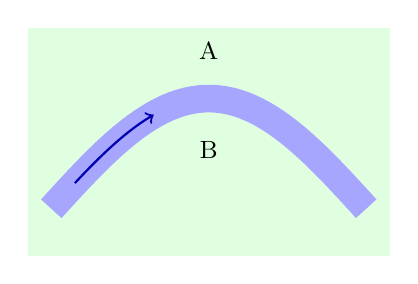
\begin{tikzpicture}[x=1cm, y=1cm, font=\small]
  \fill[green!12] (-0.3,-0.6) rectangle (4.3,2.3);
  \draw[blue!35, line width=10pt] plot[domain=0:4, samples=50]
    (\x,{1.4*sin(\x*45)});
  \draw[blue!70!black, ->, thick] plot[domain=0.3:1.3, samples=20]
    (\x,{1.4*sin(\x*45)});
  \node at (2,2.0) {A};
  \node at (2,0.75) {B};
\end{tikzpicture}
\end{center}
¿En qué orilla, A o B, desgasta el \omterm{def:g1:landscapes-around-us:water}{río} la tierra? ¿En qué orilla deja
\omterm{def:g3:stones-pebbles-sand:sand}{arena}?
\end{exercise}

\begin{exercise}[$\star$]\label{exo:g5:water-shapes-the-land:6}
En las \omterm{def:g1:landscapes-around-us:landform}{montañas}, el lecho de un \omterm{def:g1:landscapes-around-us:water}{río} está cubierto de piedras grandes. Cerca
del \omterm{def:g2:water-on-earth:ocean}{mar}, está cubierto de \omterm{def:g3:stones-pebbles-sand:sand}{arena} y \omterm{def:g3:stones-pebbles-sand:sand}{barro}. ¿Por qué?
\end{exercise}

\begin{exercise}[$\star\star$]\label{exo:g5:water-shapes-the-land:7}
Un \omterm{def:g1:landscapes-around-us:water}{río} mide 600 kilómetros de largo. Su curso alto es el primer
$\frac{1}{6}$ de su longitud, y su curso medio, el $\frac{1}{2}$
siguiente.
\begin{enumerate}
  \item[(a)] ¿Cuánto mide el curso alto? ¿Y el curso medio?
  \item[(b)] ¿Cuánto mide el curso bajo? ¿Qué fracción del \omterm{def:g1:landscapes-around-us:water}{río} es?
\end{enumerate}
\end{exercise}

\begin{exercise}[$\star\star$]\label{exo:g5:water-shapes-the-land:8}
Vuelve a mirar la fotografía del \omterm{def:g1:landscapes-around-us:water}{río} Mamoré vista desde la estación
espacial, en la página~\pageref{fig:g5:water-shapes-the-land:mamore}. ¿Qué
son las manchas claras de la parte de dentro de las curvas? ¿Qué son los
\omterm{def:g1:landscapes-around-us:water}{lagos} curvos oscuros que hay junto al \omterm{def:g1:landscapes-around-us:water}{río}? ¿Cómo se formaron?
\end{exercise}

\begin{exercise}[$\star\star$]\label{exo:g5:water-shapes-the-land:9}
Un pueblo quiere construir un colegio nuevo en los prados verdes y llanos
que hay junto a su \omterm{def:g1:landscapes-around-us:water}{río}, porque allí el terreno es llano y barato. ¿Qué le
dirías al ayuntamiento? Usa las palabras \emph{\omterm{def:g5:water-shapes-the-land:flood}{inundación}} y \emph{\omterm{def:g5:water-shapes-the-land:flood}{llanura
de inundación}}.
\end{exercise}

\begin{exercise}[$\star\star$]\label{exo:g5:water-shapes-the-land:10}
Los \omterm{def:g1:landscapes-around-us:water}{ríos} del mundo llevan al \omterm{def:g2:water-on-earth:ocean}{mar} unos 12\,000 millones de toneladas de
\omterm{def:g3:stones-pebbles-sand:sand}{barro} y \omterm{def:g3:stones-pebbles-sand:sand}{arena} cada año.
\begin{enumerate}
  \item[(a)] ¿Cuántas toneladas son cada mes, de media?
  \item[(b)] Un camión grande lleva 10 toneladas. ¿Cuántos viajes de camión
        harían falta para llevar el \omterm{def:g3:stones-pebbles-sand:sand}{barro} y la \omterm{def:g3:stones-pebbles-sand:sand}{arena} de un mes?
\end{enumerate}
\end{exercise}

\begin{exercise}[$\star\star\star$]\label{exo:g5:water-shapes-the-land:11}
Cuenta la historia de un grano de \omterm{def:g3:stones-pebbles-sand:sand}{arena}. Empieza formando parte de una \omterm{def:g3:stones-pebbles-sand:rock}{roca}
en lo alto de una \omterm{def:g1:landscapes-around-us:landform}{montaña} y termina, muchos años después, en un \omterm{def:g5:water-shapes-the-land:delta}{delta}. Usa
las palabras \emph{\omterm{def:g5:water-shapes-the-land:weathering}{meteorización}}, \emph{\omterm{def:g5:water-shapes-the-land:erosion}{erosión}} y \emph{\omterm{def:g5:water-shapes-the-land:deposition}{sedimentación}}, y
di qué le pasa al grano en el curso alto, en el curso medio y en el curso
bajo del \omterm{def:g1:landscapes-around-us:water}{río}.
\end{exercise}
